\section*{Metodologia badań}
\addcontentsline{toc}{section}{Metodologia badań}
W tym rozdziale przedstawiono metodologię przeprowadzonych badań, środowisko testowe oraz wybrane algorytmy do badań środowisk uruchomieniowych.

\section*{Środowisko testowe}
\addcontentsline{toc}{subsection}{Środowisko testowe}
Do przeprowadzenia testów został wykorzystany system operacyjny Linux Ubuntu 22.04.03, zainstalowany w (ang. \textit{ang. Windows Subsystem for Linux}). Wybór ten dodatkowo jest podyktowany faktem iż do momentu pisania niniejszej pracy, środowisko Bun nie udostępniło oficjalnego wsparcia dla systemu Windows.

Wybór powyższego systemu jest podyktowany faktem, że jest to system, na którym wybrane środowiska są najczęściej uruchamiane. Badanie wykonane w 2015 roku, pokazuje iż większość osób odpowiedzialnych za administrowanie aplikacjami webowymi korzysta z systemu Linux \cite{performance_comparison_linux}. Kolejnym badaniem przeprowadzonym w 2021 roku, pokazało iż sam system jest bardziej wydajny niż Windows Server \cite{web_server_performance}. Badania także pokazało, że większość serwerów internetowych działa na systemie Linux. W związku z tym, wybór systemu Linux jest uzasadniony.

Wymienione środowiska posługują się swoimi implementacjami programów umożliwiających uruchamianie programów opartych o Javascript, staje się to problematyczne w przypadku użycia języka TypeScript. Aby uruchomić skrypty napisane za pomocą tego języka TypeScript należy je stranspilować do języka Javascript. W przypadku NodeJs, powstały odpowiednie paczki tj.: \textit{ts-node} \cite{ts_node}, \textit{tsx} \cite{tsx}. Potrafią one przetworzyć pliki napisane w TypeScript do Javascript. W przypadku Deno oraz Bun, ta funkcjonalność jest wbudowana w środowisko, pozwala to na zrezygnowanie z dodatkowych narzędzi.

Środowiska także inaczej podchodzą do zapisu plików na urządzeniach. We wszystkich środowiskach można zapisać oraz odczytać plik za pomocą metod synchronicznych jak i asynchronicznych. Środowisko Bun udostępnia swoją implementacje zapisy oraz odczytu wykorzystując swoje metody asynchroniczne. Dodatkowym atutem samego środowiska Bun jest możliwość użycia bibliotek, które są odpowiednikiem dla tych dostępnych w NodeJs. W przypadku Deno, zapis oraz odczyt odbywa się za pomocą dekoderów oraz enkoderów, które odczytują tekst w zadanym formacie.

\section*{Wybrane narzędzi i algorytmy}
\addcontentsline{toc}{subsection}{Wybrane algorytmy}
W tym rozdziale znajdują się algorytmy wykorzystane w testach wydajnościowych dla każdego środowiska uruchomieniowego. Wraz z podaniem opisu algorytmu, znajduje się także opis zastosowania algorytmu w praktyce.

\section*{Algorytmy sortowania}
\addcontentsline{toc}{subsubsection}{Algorytmy sortowania}
W testach zostały wykorzystane trzy algorytmy sortowania, które są najczęściej wykorzystywane w praktyce. Sortowanie jako metoda jest używana w wielu zastosowaniach, takich jak sortowanie danych w bazach danych, sortowanie danych w aplikacjach webowych, a także w algorytmach wyszukiwania. W teście sortowania został przeprowadzone testy na sortowaniu danych liczbowych.

Każdy z algorytmów charakteryzuje się inną złożonością obliczeniową, co wpływa na czas sortowania danych. Możemy to zauważyć w pracy \cite{sorting}, gdzie pokazywane są czasy poszczególnych algorytmów sortowania. W tabeli \ref{tab:sorting_complexity} przedstawiono złożoności obliczeniowe dla poszczególnych algorytmów.

\begin{table}[h]
  \centering
  \begin{tabular}{|l|l|l|l|}
  \hline
  \textbf{Algorytm Sortowania} & \textbf{Optymistyczna} & \textbf{Średnia} & \textbf{Pesymistyczna} \\ \hline
    Bubble Sort & O(n) & O($n^2$) & O($n^2$) \\ 
    \hline
    Quick Sort & O(n log n) & O(n log n) & O($n^2$) \\ 
    \hline
    Radix Sort & O(nk) & O(nk) & O(nk) \\
    \hline
  \end{tabular}
  \caption{Złożoność obliczeniowa dla algorytmów sortowania}
  \label{tab:sorting_complexity}
\end{table}


\section*{Algorytmy Kodowania}
\addcontentsline{toc}{subsubsection}{Algorytmy Kodowania}
W testach został wykorzystany jeden algorytm kodowania, który jest najczęściej wykorzystywany do przesyłania danych. Wybrany algorytm kodowania jest Base64. Wykorzystywany jest on do kodowania obrazów, danych wykorzystywanych w formularzach, a także do przedstawiania plików pdf na stronach.

Algorytm możemy podzielić na trzy etapy. Pierwszym etapem jest podział danych na segmenty składające się z 24 bit. Następnie każdy z segmentów jest dzielony na cztery grupy po 6 bitów. Każda grupa zostaje mapowana na z jeden ze znaków:
\begin{itemize}
  \item Litery A-Z (26 znaków)
  \item Litery a-z (26 znaków)
  \item Cyfry 0-9 (10 znaków)
  \item Znaki "+" i "/"
\end{itemize}
W przypadku gdy grupy nie są wielokrotnością liczby 24, wtedy grupy zostają uzupełnione zerami, co przekształca się w znak \textit{=} w celu wskazania liczby dodanych bitów. Na rys \ref{fig:base64_mapping_table} przedstawiono tablicę mapowań dla algorytmu szyfrowania Base64.

\begin{figure}[H]
  \centering
  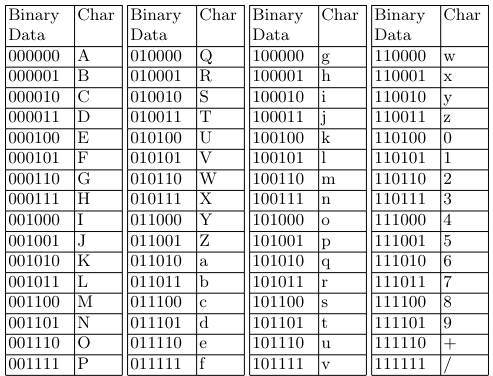
\includegraphics[width=0.6\textwidth]{Figures/base64_mapping_table.png}
  \caption{Tablica mapowań dla algorytmu szyfrowania Base64}
  \label{fig:base64_mapping_table}
\end{figure}

Algorytm ten jest przydatny do małych obrazów, jednakże w przypadku dużych obrazów, algorytm ten nie jest zalecany. Wynika to z faktu iż sam algorytm powoduje zwiększenia rozmiaru danych. Dodatkowo wykazano, że w zależności od języka programowania oraz implementacji algorytmu, czas kodowania oraz dekodowania może się różnić \cite{cryptoeprint:2022/361}.

Test został zaimplementowany z wykorzystaniem obiektu \textit{Buffer} odpowiedzialnego za kodowanie oraz dekodowanie wartości zakodowanych wiadomości. Oryginalny test wykonany przez Kostya \cite{base64_benchmark}, został zmodyfikowany, aby dodać informacje o czasie wykonywania oraz użyciu pamięci przez dane środowisko. Test ten został przeprowadzony w celu sprawdzenia jak szybko dane środowisko jest w stanie zakodować oraz odkodować dane.

\subsection*{Bazy danych}
\addcontentsline{toc}{subsubsection}{Bazy danych}


\section*{Narzędzia pomiarowe}
\addcontentsline{toc}{subsection}{Narzędzia pomiarowe}
